\chapter{Particles and The Large Hadron Collider}
\label{sec:particleslhc}

\section{The Standard Modell}
\label{sec:sm}

The standard model of particle physics describes the known elementary particles and their interactions. It consists of 12 matter particles, the fermions
and five interaction particles, which are called vector bosons. The
fermions can be grouped in two categories, six quarks and
six leptons. The quarks as well as the leptons are divided into three generations.
Each matter particle also has an antiparticle, with an opposite charge.
The interactions are obtained from the vector bosons mentioned above.
The three potent interactions are the electromagnetic(em) interaction,
the weak interaction and the strong interaction. Gravitation does not make a significant contribution.
The vector boson of the em interaction is the photon which is exchanged between particles.
% here, a feynman diagram would be nice. as well as for every other force
The strength of one of those interactions is
described by a coupling constant. In the em interaction this is the
fine structure constant\cite{alphas}. The range of the em-interaction is in principle
infinite, but decreases with increasing distance between the interacting particles.
The em interaction is described by quantum electrodynamics.
The potentials are described by operators, which create and annihilate the photons.

The exchange particles of the weak interaction are on the one hand the $W^{\pm}$-bosons and on the other hand the Z-boson.
The weak interaction processes are called currents.
Changing the charge during the interaction by a W-boson is called charged current.
The exchange reaction of a Z boson in, for example, processes such as $e_{\nu} \mu \to e_{\nu} \mu$ is called neutral current.
Analogous to the electromagnetic interaction, the potentials are again understood as
operators, but here there are no propagators. Propagators are
used in \textit{FEYNMAN}-diagrams of QED to represent the interaction particles.
A so-called V-A structure is used here instead. Here, V stands for vectorboson and A is the axialvector.
This structure is needed to disregard the right-handed particles and left-handed
antiparticles, since these lead to the charge-parity violation. Thus one adjusts the Lorentz factors in the following way
\begin{equation*}
  \gamma_{\mu} \to \gamma_{\mu}(1 - \gamma_5)
\end{equation*}
In the strong interaction, the exchange particles are the eight different
gluons. The strong interaction is described by quantum chromodynamics (QCD).
According to this, color is transfered during the interaction. Gluons
have no mass and are spin-1 particles. Gluons carry a color and a different anti-color. Gluons can also couple to themselves. Moreover, the coupling constant $\alpha_s \approx 0.1$. The interaction with quarks is described with a potential.
\begin{align}
  \symup{V}_{q\bar{q}} &= -\frac{4 \alpha_{s}}{3 r} + \sigma\cdot r
  \intertext{mit}
  \sigma &= \SI{1}{\giga\electronvolt\per\femto\metre}
\end{align}
Quarks thus tend to attract each other very strongly. If now
quark and antiquark are moved away from each other, a lot of energy has to be expended. This energy can become so large that new particles can be created.

% now particles
The standard model houses 12 spin-$\frac{1}{2}$ fermions. Six are called leptons and they are sorted into three families, also called falvor (e, μ and τ). Each of those families has a charged lepton\footnote{can have both h\"ndigkeiten} and a left-handed neutrino.
A particle is called left-handed if its spin direction is opposite to the direction of flight.cRight-handed particles have a spin direction pointing with the direction of flight. Therefore, a left-handed isospin doublet and a right-handed singlet is constructed.
The leptons can couple via the weak-interaction and if they are charged, also via the em-interaction. Neutrinos can only couple via the weak interaction.

The quarks are spin-$\frac{1}{2}$-fermions and carry an electric charge as well. In each of the three generations there is one isospin doublet. The quarks are ordered by ascending mass. In the first generation are the two lightest quarks,
up- and down quark, in the second generation the charm- and strange quark and
in the third generation the top- and bottom quark doublet.
Quarks carry a color charge, red, green or blue, which is an artificially introduced degree of freedom to guarantee the distinguishability.
Quarks couple via the strong interaction which is described by the quantum chromodynamic (QCD). The Eichgroup of the QCD is $SU\left(N = 3\right)$ where N is the number of introduced colors. The number of generators is therefore $N^2 -1 = 8$.
The generators are called gluons and they carry "color" and "anticolor".
The common eight gluon-wavefunctions are
\begin{align*}
  \psi_1 &= |r\bar{g}> & \psi_2 &= |r\bar{b}> \\
  \psi_3 &= |g\bar{r}> & \psi_4 &= |g\bar{b}> \\
  \psi_5 &= |b\bar{r}> & \psi_6 &= |b\bar{g}> \\
  \psi_7 &= \frac{1}{\sqrt{2}}\left(|r\bar{r}> - |g\bar{g}>\right) & \psi_8 &= \frac{1}{\sqrt{6}}\left(|r\bar{r}> + |g\bar{g}> - 2|b\bar{b}>\right) \\
\end{align*}
% hier zitieren wo ich das her hab. besser nicht wikipedia!
The second wavefunction describes a gluon interaction with a blue quark and changing the color to red.

Due to the Confinement, quarks cannot exist alone. Instead they form bonding states, so called hadrons. On the one hand there are the mesons, which consist of a quark
and an antiquark.

\begin{equation}
	|\symup{M}\!> = | q\, \bar{q}'\!>
\end{equation}

These may be from the same family (i.e. [u,d], [c,s], [t,b]), or from
different families. Mesons have a baryon number of 0. Accordingly, quarks carry the baryon number $\frac{1}{3}$. The quarks constructing a meson therefore carries color and the corresponding anticolor.
The second type are baryons. The content consists of either three quarks or
three antiquarks. However, it cannot be that one quark and two antiquarks
and vice versa occur, because baryons must have the baryon number $\symup{B} = 1$. Because baryons are stable final states as well as the mesons, the sum of their quark colors must be white. Therfore, every (anti)color must occur once in a baryon.

\begin{align}
	|\symup{B}\!> &= |q q' q''\!> \\
	|\symup{B}\!> &= |\bar{q} \bar{q}' \bar{q}''\!> \,
\end{align}

\section{particle decays and hadrons}
\label{sec:decays}
For you, this is because the bending and momentum of particles (and the location where they decay) is important to the way we can align things. Which sorts of particles can produce long tracks? etc.

\section{The LHC and LHCb}
\label{sec:lhcandB}

\subsection{The LHC}
The Large Hadron Collider (LHC)\cite{lhcInfo} is the most powerfull particle-accelerator on planet earth. With a circumference of $26,7\si{\kilo\metre}$ it is also the longest ring accelerator and it lies between $45\si{\metre}$ and $170\si{\metre}$ below the surface near Geneva in Swizerland. The tunnel was constructed for the LEP experiment between 1984 and 1989 and is operated by the European Organization for Nuclear Research (CERN). The LHC can produce centre of mass energies of $\sqrt{s} = \SI{13}{\tera\electronvolt}$ in proton-proton collisions during Run 2. After the upgrade the LHC will collide particles with the centre of mass energy $\sqrt{s} = \SI{13}{\tera\electronvolt}$.
An image of the accelerators and the experiments is shown in fig. \ref{fig:CERN}\cite{facilityCERN}.

\begin{figure}
  \centering
  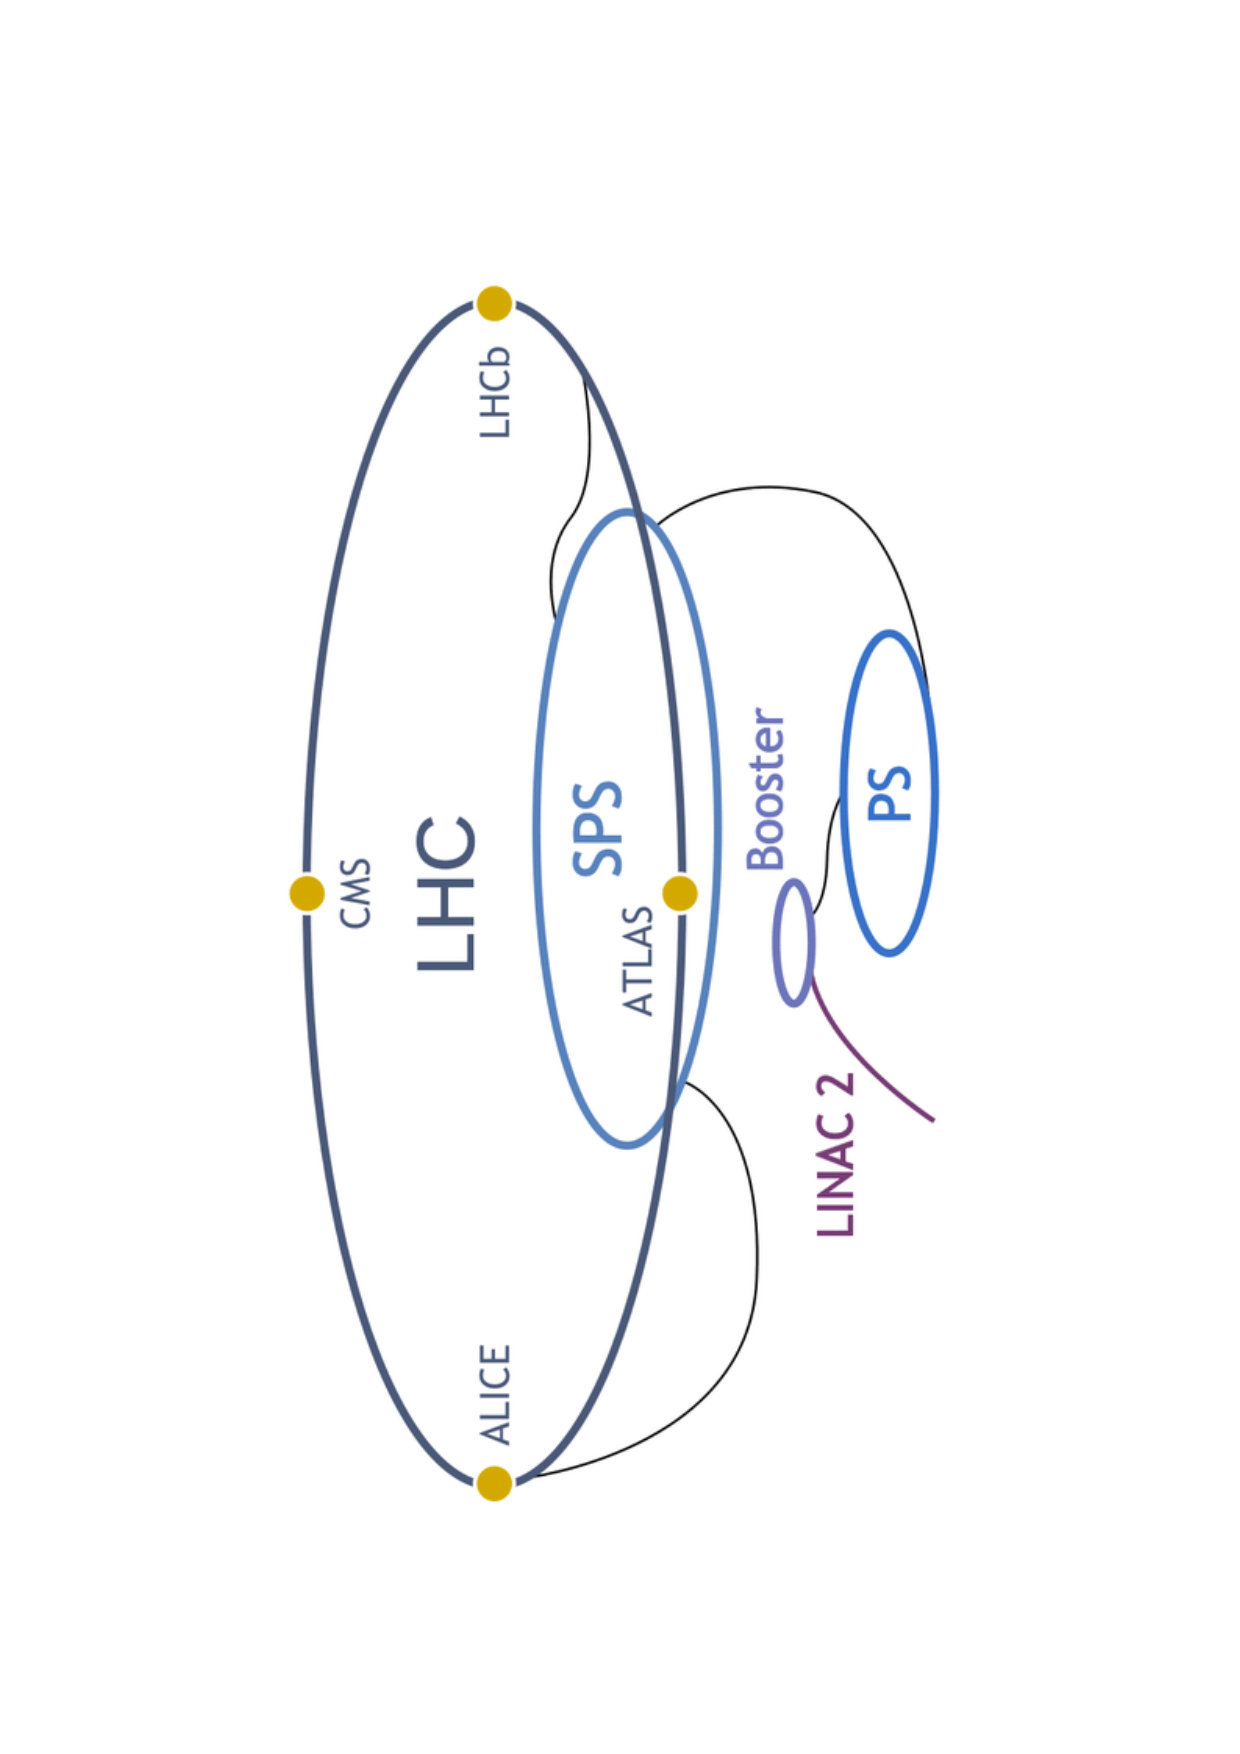
\includegraphics[angle=-90, origin=c, width=0.5\textwidth]{plots/CERN_layout.pdf}
  \caption{an overview of the LHC facilities.}
  \label{fig:CERN}
\end{figure}

By ionizing hydrogen gas, protonsare created and accelerated to $\SI{50}{\mega\electronvolt}$ by the linear accelerator (LINAC 2). Afterwards the beam is injected into the Proton Syncrotron and the Super Proton Synchrotron to a maximum of $\SI{450}{\giga\electronvolt}$ before the beam is brought into the LHC.
The beam containts several bunches with around $\num{1.15e11}$ and a bunch spacing of $\SI{25}{\nano\second}$, which is a collision rate of $\SI{40}{\mega\hertz}$.
The LHC houses four major experiments. ATLAS and CMS are classified as general purpose detectors with a detection range of close to $4\pi$. The interaction in these detectors is located in the very center so that tracks going in every direction can possibly be found. Searches for the Higgs Boson is just one of many physics aspects these detectors are build for.
The other two Experiments located at the LHC are ALICE and LHCb.
The ALICE experiment main studies the quark gluon plasma during the runs with lead ion collisions instead of protons.
In this thesis the Scintillating Fibre Tracker (SciFi Tracker) located at the LHCb will be focused at and discussed on the following chapters.

\subsection{The LHCb}

\begin{figure}
  \centering
  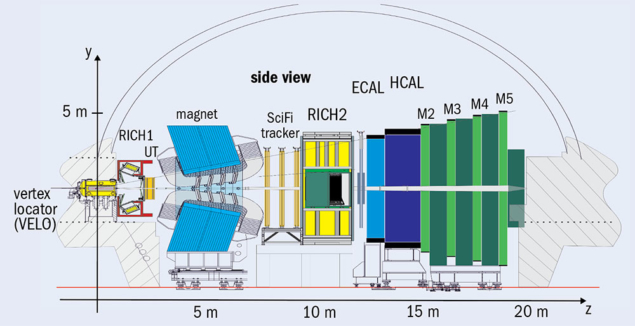
\includegraphics[width=0.5\textwidth]{plots/LHCb_facility.jpg}
  \caption{a sideview of the LHCb experiment.}
  \label{fig:LHCb}
\end{figure}

The LHCb experiment\cite{lhcbInfo} is a forward spectrometer covering $2 \less \eta \less 5$ in the pseudorapidity range. This experiments main physics goal is beauty quark physics and for high energies, b- and $\bar{b}$-hadrons are heavily produced in a tight forward direction\footnote{They are also produced in a tight backward direction but the experiment is only build for the forward cone.}. A sideview of the LHCb is shown in figure \ref{fig:LHCb}.
The LHCb consists of several smaller detector components namely the Vertex Locator (VELO) right on the intercation point, two Ring Imaging Cherenkov counter (RICH 1 and RICH 2), in front of the spectrometers lies the Trigger Tracker and behind them the SciFi Tracker which is the important part of this thesis. Further back a Scinitllator Pad Detector (SPD) and a Preshower (PS) are mounted followed by the electromagnetic calorimeter (ECAL) and the hadronic calorimeter (HCAL). In the very back, several muon chambers are mounted for every track that is yet to be determined.

In this section, a general overview about the requirements for the SciFi Tracker as well as the layout will be discribed based on the presentation in the \textit{technical design report}\cite{scifiInfo} of the upgrade.

The upstream and downstream trackers provide a good precision estimate of the momentum of charged particles so that mass resolution of decayed particles can be precisely measured. % this is a sentence i used from the TDR!
For particle identification the reconstructed trajectories of charegd particles are used as input for the RICH detectors.
The limiting factor for the momentum resolution is multiple scattering for tracks with a momentum lower than $\SI{80}{\giga\electronvolt\per\c}$. For tracks with a higher momentum the detector resolution is the limiting factor.

% why is the scifi there
The SciFi Tracker replaced the inner Tracker (IT) and the outer Tracker (OT) and is located in the same place as the downstream trackers that were previously installed.

% data and facts
The instantaneous luminosity after the upgrade is expected to be $\SIrange{1}{2e33}{\per\centi\metre\squared\per\second}$. The bunch spacing will be $\SI{25}{\nano\second}$ and the number of proton-proton interactions per bunch crossing will be $\nu = 3.8$ during the ramp-up phase of the LHC and $\nu = 7.6$ "during the active phase." (how can i write this differently?)

% layout
\subsection{Layout of the SciFi Tracker}
The SciFi Tracker consists of three (T-)stations T1, T2 and T3 with each having four layers ($X1, U, V, X2$). The orientation of these planes with respect to the vertical axis are ($\SI{0}{\degree}, \SI{+5}{\degree}, \SI{-5}{\degree}, \SI{0}{\degree}$).
The tilted layers are called stereo layers and serve the purpose of 3D hit localization.
The layers are $\SI{20}{\milli\metre}$ apart from each other in $z$-direction within each station.
Each layer has four quarters with each quarter having five\footnote{six for the last (T-)station.} modules. Each module is constructed from four fibre mats.
A right-handed coordinate system is used with positive $z$ pointing away from the interaction point following the beam direction. positive $y$ points upwards, towards the surface and positive $x$ and negative $x$ are defined as A-Side and C-Side\cite{scifiInfo}.

To ensure an optimal alignment, a well known geometry is key. Therefore, the fibres must aligned within $\SI{1}{2}{\micro\metre}$ in $x$-direction and must not be more than $\SI{300}{\micro\metre}$ bent in $z$-direction.
% here a picture of the scifi

\subsection{Scintillating Fibres}
The scintillating fibre material is a polymer with an organic flourescent dye added to the polystyrene structure to enhance the yield during the scintillation process.
In order to produce and register a photon signal, the ionisation energy is deposited in the fibre core firstly. The amount of energy need for the polymer to reach an excited state is just a few electronvolts.
The added dye has the particular structure to match the excitation energy.
The energy is transferred via the Förster Transfer.
The dye generates excited energy states when particles hit the fibre and deposit their energy. When the states relax, a photon is emitted which then excites other parts of the dye to eventually transfer the energy to the silicon photomultipliers (SiPMs) which are mounted on the outer(?) end of the mats.
The other end of the fibre mats is a full reflective mirror to send the photons towards the SiPMs.

\section{The LHC data cycle}
\label{sec:datacycle}

(not sure if that's a good name, but like, an explanation of how electrical information is turned into hits and then tracks, and also when alignment runs in the system of data taking)
